% Pulling a 1-form alpha back along a map phi: U -> U'.
% Source: book/tex/diffgeo/stokes.tex (§ Pullback of differential forms).
\documentclass[border=2mm]{standalone}
\usepackage{tikz}\usetikzlibrary{arrows.meta}\usepackage{amssymb}
\begin{document}
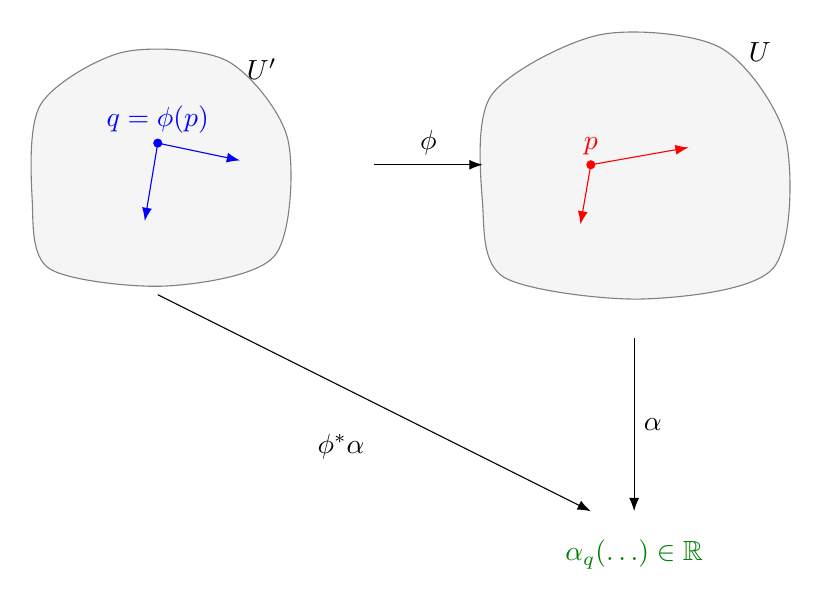
\begin{tikzpicture}[scale=0.55,>={Latex}]
  % U' on the left
  \draw[gray,fill=gray!8] plot[smooth cycle] coordinates {(-13.5,-2.4)(-10.8,-2.8)(-8.3,-2.1)(-8,0.6)(-9.4,2.4)(-11.8,2.6)(-13.7,1.4)(-13.9,-0.8)};
  \node at (-8.6,2.2){$U'$};
  \fill[blue] (-11,0.5)circle(3pt) node[blue,above]{$q=\phi(p)$};
  \draw[blue,->] (-11,0.5)--(-11.3,-1.3); \draw[blue,->] (-11,0.5)--(-9.1,0.1);
  % U on the right
  \draw[gray,fill=gray!8] plot[smooth cycle] coordinates {(-3,-2.6)(0.2,-3.1)(3.2,-2.4)(3.5,0.6)(2,2.7)(-0.8,3)(-3.3,1.6)(-3.5,-0.9)};
  \node at (2.9,2.6){$U$};
  \fill[red] (-1,0)circle(3pt) node[red,above]{$p$};
  \draw[red,->] (-1,0)--(-1.24,-1.38); \draw[red,->] (-1,0)--(1.26,0.4);
  \draw[->] (-6,0)--(-3.5,0) node[midway,above]{$\phi$};
  \draw[->] (0,-4)--(0,-8) node[midway,right]{$\alpha$};
  \node[green!50!black] at (0,-9){$\alpha_q(\dots)\in\mathbb{R}$};
  \draw[->] (-11,-3)--(-1,-8); \node[below left] at (-6,-6){$\phi^\ast\alpha$};
\end{tikzpicture}
\end{document}
